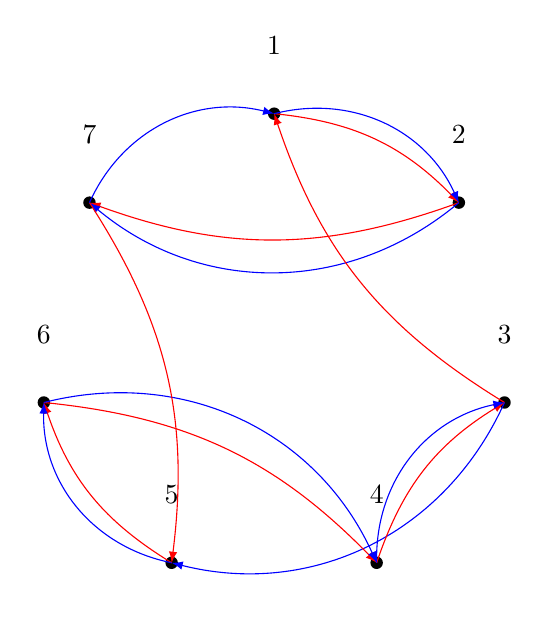
\begin{tikzpicture}[>=latex, scale=1.5]
  % Define the radius of the circle
  \def\radius{2cm}
  
  % Place the points in a circle and label them
  \foreach \i in {1,...,7} {
    % Calculate the angle for each point
    \def\angle{{90 - (\i-1)*360/7}}
    % Define the coordinate for the point
    \coordinate (N\i) at (\angle:\radius);
    % Draw a small filled circle to represent the point
    \fill (N\i) circle (1.5pt);
    % Place the label near the point
    \node[label={[shift={(0,0.5)}]$\i$}] at (N\i) {};
  }
  
  % Define the permutation sigma as a list
  \def\sigma{{2,7,1,3,6,4,5}}
	\def\tau{{2, 7, 5, 3, 6, 4, 1}}
  
  % % Draw the arrows based on the permutation
  % \foreach \i [evaluate=\i as \j using \sigma[\i-1]] in {1,...,7} {
  %   \draw[->, bend left=20] (N\i) to (N\j);
  % }
	\foreach \i in {1,...,7} {
		\pgfmathtruncatemacro{\j}{\sigma[\i-1]}
		\pgfmathtruncatemacro{\k}{\tau[\i-1]}
    \draw[->, bend left=20, red] (N\i) to (N\j);
		\draw[->, bend left=40, blue] (N\i) to (N\k);
  }
\end{tikzpicture}